\documentclass[border=4pt]{standalone}
\usepackage{tikz}
\usetikzlibrary{shapes.symbols,positioning,arrows.meta}

\begin{document}
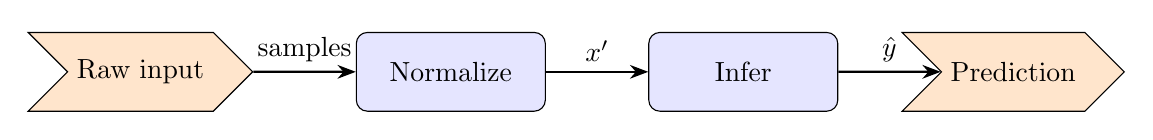
\begin{tikzpicture}[
  >=Stealth,
  node distance=13mm,
  io/.style={signal,signal from=west,signal to=east,draw,minimum width=25mm,
    minimum height=10mm,fill=orange!20},
  process/.style={draw,rounded corners,minimum width=24mm,minimum height=10mm,fill=blue!10},
  flow/.style={->,thick}
]
  \node[io] (input) {Raw input};
  \node[process,right=of input] (clean) {Normalize};
  \node[process,right=of clean] (infer) {Infer};
  \node[io,right=of infer] (output) {Prediction};

  \draw[flow] (input) -- node[above]{samples} (clean);
  \draw[flow] (clean) -- node[above]{$x'$} (infer);
  \draw[flow] (infer) -- node[above]{$\hat y$} (output);
\end{tikzpicture}
\end{document}
